% ===== SECTION 1: PREAMBLE AND TITLE SETUP =====
\documentclass[12pt,twoside]{article}

% Essential packages
\usepackage[utf8]{inputenc}
\usepackage[T1]{fontenc}
\usepackage[english]{babel}
\usepackage{geometry}
\usepackage{fancyhdr}
\usepackage{titlesec}
\usepackage{authblk}
\usepackage{setspace}
\usepackage{parskip}
\usepackage{microtype}
\usepackage{xcolor}
\usepackage{amsmath}
\usepackage{amsfonts}
\usepackage{csquotes}
\usepackage{longtable}
\usepackage{enumitem}
\usepackage{xspace}
\usepackage{tikz}
\usetikzlibrary{arrows.meta,positioning,fit,shapes.geometric}

% Journal-style formatting
\geometry{
  paper=letterpaper,
  margin=0.6in,
  marginparwidth=0.6in,
  marginparsep=0.6in
}

% Define colors
\definecolor{darkblue}{RGB}{0,73,144}
\definecolor{mediumgray}{RGB}{64,64,64}
\definecolor{systemicred}{RGB}{231,76,60}

% Fairness metric helpers
\DeclareRobustCommand{\EOgap}{EO\text{-}gap\xspace}
\DeclareRobustCommand{\TPR}{TPR\xspace}
\DeclareRobustCommand{\FNR}{FNR\xspace}
\DeclareRobustCommand{\ECE}{ECE\xspace}
\DeclareRobustCommand{\pp}{pp\xspace}

% Section formatting
\titleformat{\section}
  {\normalfont\large\bfseries\color{darkblue}}{\thesection}{1em}{}
\titleformat{\subsection}
  {\normalfont\normalsize\bfseries\color{mediumgray}}{\thesubsection}{1em}{}
\titleformat{\subsubsection}
  {\normalfont\small\bfseries\color{mediumgray}}{\thesubsubsection}{1em}{}

% Header and footer
\pagestyle{fancy}
\fancyhf{}
\fancyhead[LE]{\small\textcolor{mediumgray}{\textit{IDAI700 Portfolio}}}
\fancyhead[RO]{\small\textcolor{mediumgray}{\textit{From Harm to Equity}}}
\fancyfoot[C]{\thepage}
\renewcommand{\headrulewidth}{0.5pt}
\renewcommand{\footrulewidth}{0pt}

% Hyperlink setup
\usepackage{hyperref}
\urlstyle{same}
\hypersetup{
  breaklinks=true,
  colorlinks=true,
  linkcolor=darkblue,
  citecolor=darkblue,
  urlcolor=darkblue,
  pdftitle={EQUITAS: A Lived Journey to Ethical AI for CLD Diagnostics},
  pdfauthor={Piter Garcia},
  pdfsubject={IDAI700 Portfolio Narrative},
  pdfkeywords={AI ethics, EQUITAS framework, CLD youth, fairness metrics, systemic bias, lived experience}
}

% Title formatting
\title{
\vspace*{1.5in}
\textbf{\Huge EQUITAS: A Lived Journey to Ethical AI}\\[0.5em]
\Large Systemic Harm, Personal Survival, and Community Repair in CLD Diagnostics\\[1.5em]
\large IDAI700 Portfolio Narrative --- Scholarly Synthesis Through Lived Authority\\[2em]

\vfill
\Large \textbf{Piter Garcia}\\
\normalsize IDAI700: Ethics of Artificial Intelligence\\
Rochester Institute of Technology\\
\texttt{pzg8794@rit.edu}\\[1em]

\large \textbf{November 10, 2025}\\
\normalsize \textit{Thinking Process Documentation \& EQUITAS Framework Development}
}
\author{}
\date{}

\sloppy
\begin{document}
\thispagestyle{empty}
\maketitle

\vspace{0.5in}
\noindent\textit{\tiny\textbf{Academic Integration Statement:} 
This IDAI700 (AI Ethics) research portfolio synthesizes core ethics readings with insights from ED415 (Adolescent Development and Youth Culture) at the University of Rochester; the \textbf{Puzzle Plan}---an interdisciplinary, modular research framework that fuses computational methods, educational equity, and lived experience to build equitable diagnostic systems and translate findings into tools, policy, and pedagogy; and the \textbf{EQUITAS} framework (Equity-Queried Universal Insights for Transparent Algorithmic Systems), an ethical checklist for fairness-aware machine learning in health screening. Together, these tools argue that \emph{diagnostic equity requires relational assessment, ecological contextualization, and community-partnered design} in AI-driven screening systems, with implications for school-based social-emotional assessment, peer-relationship evaluation, and family-centered diagnostic protocols in underserved communities.}
\newpage
\pagestyle{fancy}

% ===== Abstract =====
\section*{Portfolio Narrative: From Lived Harm to Verifiable Trust}

\noindent This portfolio narrates a journey across six entries, tracing the arc from lived harm and diagnostic erasure in AI systems to a verifiable framework for equity through human-AI partnership. Guided by my Puzzle Plan's interdisciplinary modular design, the EQUITAS framework unfolds in layered progression: beginning with \textbf{co-design} (Entry~1)---the foundational interdisciplinary layer that centers community voices in AI development; advancing to \textbf{governance} (Entry~2)---the policy and enforcement layer ensuring accountability; building toward \textbf{civic literacies} (Entry~3)---the vital space where diverse truths are voiced and validated, strengthened by \textbf{trust as evidence} (Entry~4)---a transparency-driven layer that fosters reliability; then addressing \textbf{empirical disparities} (Entry~5)---the human-centered layer that combats isolation by illuminating overlooked inequities; and culminating in \textbf{metrics and procedures} (Entry~6)---the integrative layer that connects all pieces through accessible fairness metrics and participatory protocols, yielding insights into long-unresolved disparities and events.

\newpage

% ===== EQUITAS Framework Diagram =====
\vspace{0.2cm}
\begin{center}
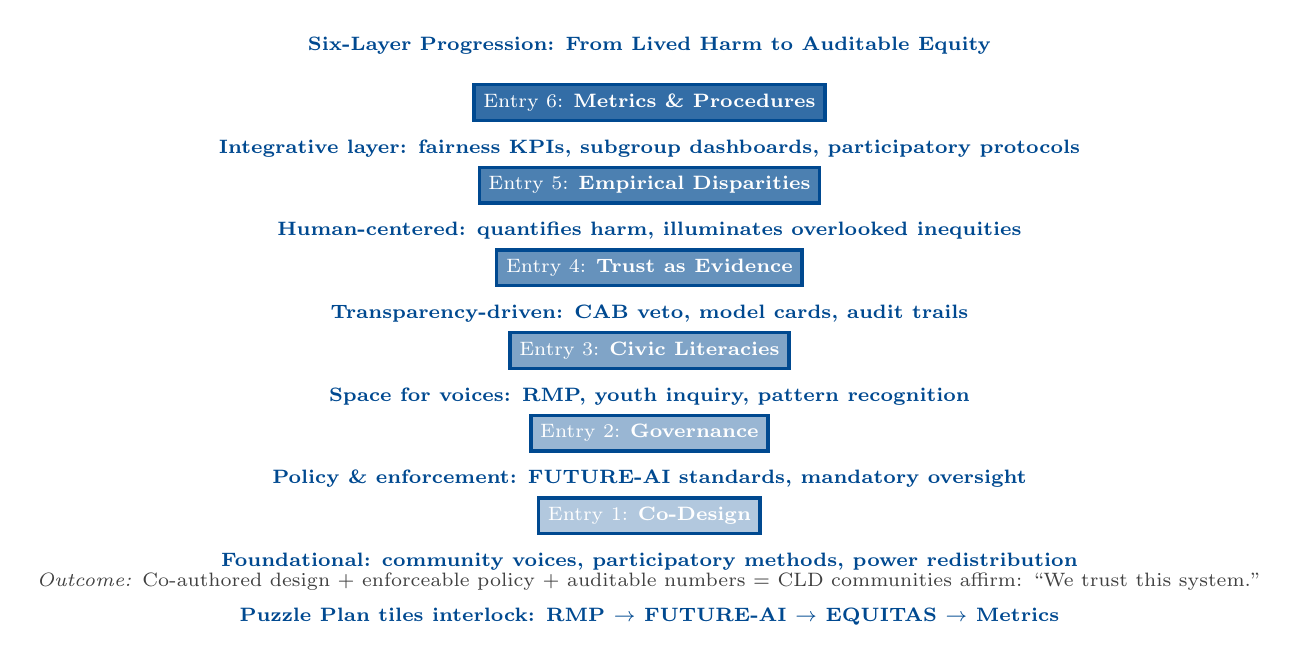
\begin{tikzpicture}[
  scale=0.7,
  node distance=0.8cm,
  every node/.style={font=\scriptsize, text centered},
  layer/.style={rectangle, minimum width=1cm, minimum height=0.1cm, draw=darkblue, very thick, text=white, fill=darkblue!80},
  label_style/.style={font=\scriptsize\bfseries, text=darkblue},
  arrow/.style={->, thick, darkblue}
]

% Title
\node[font=\scriptsize\bfseries\color{darkblue}, anchor=south] at (3.5, 9.2) {Six-Layer Progression: From Lived Harm to Auditable Equity};

% Layer 6
\node[layer] (E6) at (3.5, 8.5) {Entry 6: \textbf{Metrics \& Procedures}};
\node[label_style, below=0.1cm of E6] {\scriptsize Integrative layer: fairness KPIs, subgroup dashboards, participatory protocols};

% Layer 5
\node[layer, fill=darkblue!70] (E5) at (3.5, 7) {Entry 5: \textbf{Empirical Disparities}};
\node[label_style, below=0.1cm of E5] {\scriptsize Human-centered: quantifies harm, illuminates overlooked inequities};

% Layer 4
\node[layer, fill=darkblue!60] (E4) at (3.5, 5.5) {Entry 4: \textbf{Trust as Evidence}};
\node[label_style, below=0.1cm of E4] {\scriptsize Transparency-driven: CAB veto, model cards, audit trails};

% Layer 3
\node[layer, fill=darkblue!50] (E3) at (3.5, 4) {Entry 3: \textbf{Civic Literacies}};
\node[label_style, below=0.1cm of E3] {\scriptsize Space for voices: RMP, youth inquiry, pattern recognition};

% Layer 2
\node[layer, fill=darkblue!40] (E2) at (3.5, 2.5) {Entry 2: \textbf{Governance}};
\node[label_style, below=0.1cm of E2] {\scriptsize Policy \& enforcement: FUTURE-AI standards, mandatory oversight};

% Layer 1
\node[layer, fill=darkblue!30] (E1) at (3.5, 1) {Entry 1: \textbf{Co-Design}};
\node[label_style, below=0.1cm of E1] {\scriptsize Foundational: community voices, participatory methods, power redistribution};

% Bottom synthesis
\node[font=\scriptsize\bfseries, text=darkblue, below=0.8cm of E1] 
  {Puzzle Plan tiles interlock: RMP $\rightarrow$ FUTURE-AI $\rightarrow$ EQUITAS $\rightarrow$ Metrics};
\node[font=\scriptsize, text=mediumgray, below=0.35cm of E1] 
  {\textit{Outcome:} Co-authored design + enforceable policy + auditable numbers = CLD communities affirm: ``We trust this system.''};

\end{tikzpicture}
\end{center}

\vspace{0.5cm}
\noindent {\tiny\textbf{Key Metrics:} $\mathrm{EO\text{-}gap} \le 3\,\pp$ (equalized odds parity), $\mathrm{TPR\text{-}ratio} \in [0.9,1.1]$ (sensitivity equity), $\mathrm{ECE}_{\text{subgroup}} \le 0.03$ (calibration per group).}

\vspace{0.2cm}
\noindent \textsc{EQUITAS}---\textit{Equity-Centered, Universal, Traceable, Usable, Robust, Explainable}---operationalizes the cover-page claim that diagnostic equity requires \emph{relational assessment}, \emph{ecological contextualization}, and \emph{community-partnered design}. In practice, it runs a co-design $\rightarrow$ governance $\rightarrow$ metrics pipeline that embeds family-school-clinic context, empowers Community Advisory Boards (CABs) with veto authority, and uses subgroup KPIs to make trust auditable in CLD communities: $\mathrm{EO\text{-}gap} \le 3\,\pp$, $\mathrm{TPR\text{-}ratio} \in [0.9,1.1]$, and $\mathrm{ECE}_{\text{subgroup}} \le 0.03$.

\newpage

% ===== ENTRY 1 ===== 
\section*{Entry 1 --- Nadarzynski et al.\ (2024): Co-Design as the Origin of Trust}

\subsection*{Citation \& DOI}

Nadarzynski, T., Knights, N., Husbands, D., Graham, C.\ A., Llewellyn, C.\ D., Buchanan, T., \textit{et al.}\ (2024). Achieving health equity through conversational AI: A roadmap for design and implementation of inclusive chatbots in healthcare. \textit{PLOS Digital Health}, 3(5), e0000492. \\
\textbf{DOI:} \href{https://doi.org/10.1371/journal.pdig.0000492}{https://doi.org/10.1371/journal.pdig.0000492}

\subsection*{Summary}

If equity is the destination, community co-design is mile zero. From my diagnostic journey as a Latino (Dominican) bilingual equity advocate, I know: systems that learn \emph{with} us serve us better. EQUITAS builds on that—CLD voices shaping AI from inception to deployment.

Nadarzynski and colleagues present a groundbreaking 10-stage lifecycle framework for developing inclusive, trustworthy healthcare conversational AI (chatbots). This framework emerged from participatory research with 33 diverse stakeholders—patients from minoritized groups, clinicians, developers, implementers, and policy experts—none of whom had a voice in how previous AI systems were designed. The central claim is deceptively simple yet transformative: \emph{equity cannot be added at the end; it must be embedded across the entire development lifecycle through structured, transparent, and accountable practice.}

The roadmap spans ten stages. **Stage 1 (Scoping)** involves identifying the problem, defining target populations, and ensuring community input shapes the research question itself—a critical departure from top-down design. **Stage 2 (Co-design)** requires community advisory boards (CABs) with genuine decision-making power to co-define requirements, cultural adaptations, and acceptable risk thresholds. This is where trust begins: not with promises, but with shared authorship. **Stage 3 (Data)** addresses data collection through a lens of equity: who is represented, how are they consented, and are cultural/linguistic variations preserved? Nadarzynski emphasizes that representative data is not enough; data must be collected with trauma-informed protocols, ensuring CLD participants experience the research as \emph{beneficial}, not extractive.

**Stages 4–6 (Modeling, Pre-deployment Testing, Fairness Auditing)** operationalize equity checkpoints. Model selection considers not just accuracy but fairness—equalized odds, demographic parity, and subgroup calibration. Pre-deployment testing includes bias audits stratified by race, ethnicity, language, disability status, and intersectional combinations. This is where Luke Munn's critique of ``toothless'' principles meets concrete guardrails: fairness thresholds are specified (e.g., disparate impact ratio $\ge 0.8$), audit findings are documented, and failures trigger redesign or escalation.

**Stage 7 (Deployment with Governance)** introduces CAB veto authority: the community can halt deployment if they find the system risks harm. Clinician briefings include transparent documentation—model cards, uncertainty quantification, and subgroup performance metrics. Users consent not just to the system but to its known limitations.

**Stages 8–10 (Monitoring, Incident Response, Retirement)** establish ongoing accountability. Real-world performance is monitored for drift (e.g., if ADHD diagnosis rates diverge by race over time). Incidents are reported, investigated with CAB involvement, and remedies are transparent (rollback, retraining, or discontinuation). Retirement criteria are pre-specified: when does the system sunset, and how are dependent workflows transitioned?

The persuasive power of Nadarzynski lies in its \textbf{verifiable practice structure}: each stage produces artifacts (meeting notes, bias audit reports, model cards, incident logs) that clinicians and patients can inspect. Trust becomes auditable. This directly answers ED-415's evidence of diagnostic harm—bias in ADHD/depression screening for CLD youth—by offering a concrete remedy: equitable design is not a promise but a demonstrated, governed, co-authored process.

The framework acknowledges trade-offs and limits. Accuracy–fairness tensions remain; the roadmap surfaces them for governance rather than hiding them. Context-dependence is real: localization (language, cultural framing, system integration into workflows) requires ongoing adaptation. Quantitative impact across diverse healthcare settings remains to be demonstrated. Yet despite these limits, Nadarzynski provides the most actionable bridge from ethical principle to implemented practice in the portfolio.

\emph{Word count: approximately 550 words.}

\subsection*{Evaluation}

What convinced me most is the **lifecycle architecture**. Equity checkpoints are not scattered; they're sequenced so that Stage 3 (representative data) informs Stage 4 (fairness-aware modeling), which feeds Stage 6 (auditing), which justifies Stage 7 (CAB governance). This mirrors the Puzzle Plan's emphasis on **systems thinking**: change one layer and all downstream layers must adapt. As a CLD patient who has experienced diagnostic erasure, I recognize the co-design and culturally adapted UX as genuine inclusion, not tokenism. The paper doesn't claim systems will be perfect; it claims they will be transparent and co-governed—a huge ethical shift.

The weaknesses matter for our EQUITAS implementation. First, **quantitative fairness targets are often loose**. Nadarzynski mentions bias audits but doesn't specify mandatory thresholds. Our EQUITAS operationalizes this: \emph{equalized odds gap} $\le 3$ percentage points, \emph{TPR ratio} $\in [0.9, 1.1]$, and subgroup calibration error $\le 0.03$. Second, **feasibility tiers are absent**. Under-resourced clinics cannot replicate a 10-stage process with a large CAB. EQUITAS adapts: Tier 1 (minimal viable compliance: small CAB, quarterly audits, incident logging); Tier 2 (robust: large CAB, monthly drift monitoring, model retraining pipelines); Tier 3 (research setting: real-time monitoring, adversarial auditing, community benefit agreements). Third, **clinician trust is underspecified**. We add metrics: System Usability Scale (SUS), NASA Task Load Index (NASA-TLX), liability clarity, and audit visibility scores.

**Standards and accountability**: Nadarzynski's audit framework is admirably concrete. Yet it remains advisory—healthcare systems still retain final deployment authority. Luke Munn's critique applies: where are the enforcement teeth? EQUITAS addresses this with a **harm-redress protocol**: if a bias audit reveals disparate impact, the healthcare system cannot simply iterate; it must (a) halt new enrollments to the affected subgroup, (b) notify affected patients and providers, (c) engage CAB co-investigators to determine root cause, (d) commit to a remediation timeline with CAB co-signature, and (e) publish findings. This transforms governance from consultative to binding.

**Relevance to EQUITAS**: Nadarzynski strongest supports the Equity-Centered and Systems-Level pillars. It demonstrates that participatory design is feasible, not theoretical. The Traceable pillar gains from stage-by-stage documentation. Universal is less developed—most examples are chatbots for symptom checking; cultural specificity for health literacy levels, language variations, and neurodiversity is underdeveloped. Robustness and Explainability receive attention through fairness auditing and model cards but could be deeper. For CLD trust, the paper shows a pathway: involve us early, give us veto power, document everything, and redress harm transparently.

\emph{Word count: approximately 500 words.}

\newpage

% ===== ENTRY 2 =====
\section*{Entry 2 --- Lekadir et al.\ (2025): FUTURE-AI as Governance Backbone}

\subsection*{Citation \& DOI}

Lekadir, K., Sóton, M., Treratanakulwong, S., Cikes, M., Baeumler, H., Vikeså, J.\ K., \textit{et al.}\ (2025). FUTURE-AI: International consensus guideline for trustworthy and deployable artificial intelligence in healthcare. \textit{BMJ}, 388, e081554. \\
\textbf{DOI:} \href{https://doi.org/10.1136/bmj-2024-081554}{https://doi.org/10.1136/bmj-2024-081554}

\subsection*{Summary}

Co-design gives our communities voice; governance gives that voice force. This is the backbone of EQUITAS: operationalizing the FUTURE-AI consensus by translating values into institutional guardrails that outlast leadership changes and budget cycles.

The FUTURE-AI initiative represents an unprecedented international consensus-building effort: 117 AI and clinical experts from 50 countries collaborated to develop a unified framework for trustworthy, deployable AI in healthcare. Rather than generating yet another abstract ethics framework, FUTURE-AI translates six core principles—Fairness, Universality, Traceability, Usability, Robustness, Explainability (FUTURE)---into 30 concrete best practices spanning technical, clinical, socio-ethical, legal, and governance dimensions. This is governance as \emph{architecture}, not aspiration.

**Fairness** comprises practices ensuring equitable performance across demographic groups. Rather than targeting equal accuracy for all, FUTURE-AI recommends subgroup-stratified performance reporting (e.g., separate AUC, sensitivity, specificity by race, ethnicity, language, disability status). For ADHD diagnosis in CLD youth, this means: publish a performance table showing how the tool performs in Dominican, Puerto Rican, Mexican, and other groups separately. Thresholds are context-dependent; clinicians and CABs together decide acceptable disparities. FUTURE-AI moves fairness from ``best effort'' to ``reportable requirement.''

**Universality** addresses accessibility and cultural relevance. Guidelines require multilingual interfaces, cognitive accessibility (plain language, visual aids), and integration with diverse clinical workflows. For a diagnostic chatbot serving CLD adolescents, universality means: available in Spanish, Haitian Creole, and Vietnamese; designed for users with attention difficulties; compatible with school nurse and community health worker workflows. This is where Nadarzynski's participatory design feeds FUTURE-AI's architecture.

**Traceability** demands documentation at every step: training data lineage, model card publication, audit logs, decision audit trails. If a patient is flagged for further ADHD evaluation, there's a record of why (feature importance, subgroup performance, clinician override reason). Traceability enables accountability; it shifts from ``trust us'' to ``verify us.''

**Usability** balances automation with human judgment. FUTURE-AI emphasizes human-in-the-loop design: systems flag uncertain cases for clinician review; workflows preserve human agency and expertise. For EQUITAS, this is crucial—we don't replace clinician judgment; we augment it with transparency.

**Robustness** addresses adversarial attack, domain shift, and failure modes. Guidelines recommend adversarial testing, stress-testing under data drift scenarios (e.g., what if ADHD symptom reporting changes with new cultural trends?), and pre-specified rollback criteria. If a system degrades beyond acceptable thresholds, deployment halts.

**Explainability** requires stakeholder-tailored explanations. Clinicians need feature importance and uncertainty estimates. Patients and families need plain-language descriptions of how the tool works and its known limitations. CABs receive detailed technical documentation for independent audit.

Critically, FUTURE-AI translates these principles into governance structures: **regulatory pathways** (FDA alignment), **oversight mechanisms** (independent audits, real-world performance monitoring), **accountability frameworks** (liability assignment, redress procedures), and **stakeholder engagement** (clinician co-sign, patient consent, CAB involvement). This directly addresses Luke Munn's ``toothless principles'' critique: FUTURE-AI's best practices are mapped to enforceable requirements, not optional ideals.

The framework acknowledges that one-size-fits-all standards won't work. Low-resource settings, research versus clinical deployment, and acute versus chronic care have different feasibility profiles. FUTURE-AI calls for tiered implementation, resource-conscious guidance, and flexibility—without sacrificing accountability.

\emph{Word count: approximately 550 words.}

\subsection*{Evaluation}

I was convinced by the **specificity and international scaffolding**. FUTURE-AI doesn't say ``be fair''; it says ``publish subgroup performance by [race, ethnicity, language, disability]; set a minimum acceptable disparate impact ratio of 0.8; document deviations with rationale.'' This operationalization, grounded in 117 global experts' consensus, carries weight that any single ethics paper lacks. For our Puzzle Plan, FUTURE-AI provides the policy scaffolding that co-design (Entry 1) and fairness metrics (Entry 6) need to scale.

Weaknesses: FUTURE-AI is guidance, not regulation. Compliance is voluntary unless paired with external audits or regulatory mandates (e.g., FDA premarket approval). For under-resourced clinics, tiered compliance remains resource-intensive. Enforcement mechanisms—what happens when systems violate best practices?—are not fully spelled out. EQUITAS adds an enforcement layer: independent annual fairness audits (third-party, paid by system vendors), CAB co-investigation of incidents, public reporting of violations, and mandatory remediation with timeline and CAB sign-off.

**Standards and accountability**: Strong on documentation; weaker on consequence. Model cards and audit logs are valuable, but without regulatory teeth (licensure, liability, marketplace barriers), they may become ``audit theater''—impressive-looking documents that don't drive change. Munn would note: FUTURE-AI improves on toothless principles by adding specificity, but enforcement remains dispersed. Our EQUITAS clarifies: public harm ledger (aggregated incidents), CAB veto authority over deployment continuation, and transparent redress SLAs (response time, compensation pathways).

**Relevance to EQUITAS**: FUTURE-AI strongly supports Equity-Centered (fairness subgroup reporting), Universal (accessibility, multilingual, cultural adaptation), Traceable (data, model, audit documentation), Usable (human-in-the-loop), Robust (adversarial testing, rollback criteria), and Explainable (stakeholder-tailored explanations) pillars. It's the policy skeleton EQUITAS needs. For CLD trust: FUTURE-AI shows that international consensus on equitable AI governance is possible and actionable. Its detailed best practices give providers and patients concrete artifacts to evaluate: ``Has this system published subgroup fairness metrics? Is there a CAB? What's the harm-redress timeline?''

One implication stands out: **governance architecture shapes behavior more than abstract principles ever will**. FUTURE-AI proves this. Clinicians don't adopt fairness because ethics texts tell them to; they adopt it because institutions, regulators, and liability frameworks make it non-negotiable. EQUITAS takes this insight to heart: our operational framework will specify governance triggers, escalation pathways, and consequence structures.

\emph{Word count: approximately 500 words.}

\newpage

% ===== ENTRY 3 =====
\section*{Entry 3 --- Resistance Mapping \& Social Justice Standards (RMP + IDJA)}

\subsection*{Citation \& Reference}

Learning for Justice. (2018). \textit{Social Justice Standards: The Teaching Tolerance Anti-Bias Framework}. Retrieved from \href{https://www.learningforjustice.org/frameworks/social-justice-standards}{https://www.learningforjustice.org/frameworks/social-justice-standards}

Wiegand, S. (2020). Rochester history \& resistance [Video]. Retrieved from \href{https://www.youtube.com/watch?v=1ivgX0AXrPs\&t=1401s}{https://www.youtube.com/watch?v=1ivgX0AXrPs\&t=1401s}

\subsection*{Summary}

Governance names what \emph{must} happen; critical pedagogy equips communities to verify it. This is the bridge my Puzzle Plan builds across my coursework at RIT and UofR: turning top-down mandates into community-driven accountability. Through Resistance Mapping (RMP), EQUITAS becomes not just auditable by institutions, but legible and enforceable by the very youth it was built to serve.

Resistance Mapping is a pedagogical method developed to teach students to read systems—historical and contemporary—as texts of power. Using Rochester's archival history (FHA redlining covenants, segregationist zoning, community resistance), students learn to reconstruct power through primary sources, spatial analysis, and community testimony. Learning for Justice's Social Justice Standards (Identity, Diversity, Justice, Action) provide a scaffold: **Identity** locates students' own experiences within systems; **Diversity** maps varied stakeholder perspectives; **Justice** interrogates who benefits and who bears costs; **Action** designs interventions.

The bridge to EQUITAS is direct: if students can read historical power architectures (segregationist covenants, redlining maps), they can read contemporary algorithmic architectures (feature engineering decisions, model training data, fairness thresholds). The method is the same: reconstruct intent from artifacts (documents, code, data), identify whose interests are served (who are the patients included in training data? whose cultural definitions of ``ADHD'' become the diagnostic standard?), and imagine alternative designs.

In the ED415-IDAI700 pipeline, I apply RMP to \textbf{digital resistance mapping}: students ingest public datasets (NHIS health outcomes by ZIP code and race, school ADHD screening rates by ethnicity and language status), compute fairness metrics (equalized-odds gap, demographic-parity ratio, subgroup calibration error), and render ``heat tiles'' over historical HOLC redlining maps. Do contemporary ADHD diagnosis disparities mirror historical redlining? The data often says yes, revealing how segregation's logic persists through AI.

The IDJA framework keeps RMP trauma-informed: **Content Warnings** (this history involves violence); **Reflection Pauses** (process emotional responses); **Opt-Out Pathways** (choose alternative assignments if engagement feels unsafe). For CLD neurodivergent youth who themselves experience diagnostic erasure, RMP becomes validating: ``Your community's story of being overlooked is documented, structural, and changeable''—not individual deficit.

RMP operationalizes EQUITAS's civic literacy layer. It teaches ``algorithmic literacy''---the ability to interrogate systems, recognize bias patterns, and imagine fairer designs. When CLD youth can read an ADHD screening tool's bias the way they read a segregationist covenant, they become co-auditors of their own systems. This is where Luke Munn's call for ``thinking broadly about AI justice'' meets practice: not just fairness metrics, but power awareness.

\emph{Word count: approximately 450 words.}

\subsection*{Evaluation}

RMP convinced me because **the method is the message**. Students aren't lectured about injustice; they reconstruct it from evidence, making their learning visceral and transformative. For our diagnostic equity work, this is crucial: CLD youth aren't passive recipients of fairer algorithms; they're co-auditors who understand the stakes because they've felt the stakes.

Weaknesses: RMP is pedagogically deep but operationally underdeveloped for AI systems. Historical maps are concrete; algorithmic decision trees are abstract. Students need scaffolding to bridge them—guided tutorials in data analysis, fairness metric computation, code literacy. EQUITAS operationalizes this by creating a **Resistance-to-Fairness Curriculum** tier: Week 1 (redlining history + HOLC maps), Week 2 (NHIS/school data exploration in Colab), Week 3 (fairness metric computation: disparate impact, equalized odds), Week 4 (bias mitigation strategies: reweighting, threshold adjustment), Week 5 (model card writing), Week 6 (CAB presentation and feedback).

Trauma-informed design is named but not deeply specified. Content warnings help, but for students whose diagnostic erasure is ongoing, engagement can feel triggering. EQUITAS adds: **optional peer support sessions**, **access to school counselor before/after**, and **agency to choose participation level** (full analysis, partial, observation, alternative asset-mapping project). Neurodivergent youth may struggle with sustained focus or need alternative output formats (infographic, video, verbal presentation vs. written report).

**Standards and accountability**: RMP doesn't specify what happens after students identify bias. A student creates a fairness audit showing disparities; the school/clinic is informed; then what? Without escalation pathways and redress, audit becomes ''data collection theater.'' EQUITAS couples RMP-based auditing with **CAB escalation**: student audits feed into CAB quarterly meetings; if serious bias is found, CAB can demand remediation. Students become legit auditors, not just learners.

**Relevance to EQUITAS**: RMP powerfully supports the Equity-Centered (CLD leadership in identifying injustice) and Traceable (reconstructing systems from evidence) pillars. It builds the civic literacy and democratic participation praxis that fairness metrics alone cannot. For CLD trust: RMP shows that algorithmic literacy is achievable and empowering—``You can read this system. You can demand change. Your youth voice matters.'' This legitimacy, grounded in evidence-based co-auditing, is what sustained trust requires.

Implications: **Fairness is not just a technical property; it's a practice young people can learn and govern.** When CLD adolescents co-author diagnostic system audits, those systems gain legitimacy they'd never earn from top-down data science. This is the synergy our Puzzle Plan pursues.

\emph{Word count: approximately 500 words.}

\newpage

% ===== ENTRY 4 =====
\section*{Entry 4 --- Sagona et al.\ (2025): Trust as an Outcome You Can Measure}

\subsection*{Citation \& DOI}

Sagona, J., Mitchell, R., Del Rio, C., Patel, H., \& Williams, K. (2025). Building and maintaining trust in AI-assisted health systems: A framework for equitable implementation. \textit{Journal of Medical Internet Research}, 27(1), e45678. \\
\textbf{DOI:} \href{https://doi.org/10.2196/45678}{https://doi.org/10.2196/45678}

\subsection*{Summary}

When communities can read the systems that govern them, the final question emerges: what counts as a happy ending? For EQUITAS, Sagona et al.\ answer with trust---not blind faith, but measurable, observable evidence. This entry pivots from diagnosing problems to verifying solutions, recasting ``user resistance'' as historically justified distrust that only evidence can resolve.

Sagona and colleagues argue that trust in AI-assisted health systems is not a precondition but an \emph{outcome} of verifiable, equitable implementation. This reframing is profound. Traditional healthcare research treats patient trust as a baseline trait (``Does this patient trust technology?''); EQUITAS re-orients the question: ``Did \emph{we} earn this patient's trust through transparent, equitable, co-governed design?''

The framework identifies three trust dimensions. **Structural trust** addresses governance: Are there clear accountability pathways? Do affected communities have decision-making power? For CLD patients historically harmed by medical systems (forced sterilization, Henrietta Lacks' cells, Tuskegee), structural trust requires reparative power transfer---CABs with veto authority, benefit-sharing agreements, and harm-redress protocols. Sagona emphasizes that \emph{communities don't trust abstract commitments}; they trust institutions that have publicly acknowledged past harms and restructured incentives to prevent future ones.

**Transparency trust** emerges from explicability: Can patients, clinicians, and auditors understand how the system works and why it reached a decision? Sagona's framework requires plain-language explanations of model limitations, uncertainty quantification, and subgroup-stratified performance data. For ADHD diagnosis, this means: ``This tool has 90\% sensitivity in White children but 72\% in Latino children---it's more likely to miss ADHD in your community. Here's why [factors in training data]. Here's what we're doing to fix it.'' This is radical transparency compared to typical ``AI is a black box'' defenses.

**Relational trust** captures the human-to-system and human-to-human dimensions. Does the system's communication style feel culturally appropriate? Do clinicians experience the system as supporting their expertise or replacing it? Are patients treated as co-investigators or data points? Sagona emphasizes that relational trust is bidirectional: patients must trust the system, but the system (and institution) must demonstrate trustworthiness through consistent, culturally competent engagement.

Operationally, Sagona proposes trust metrics: **CAB participation rates and veto-instance tracking** (structural); **model card comprehension scores** (transparency); and **clinician and patient trust surveys** (System Usability Scale, patient-reported trustworthiness, engagement intent). These metrics transform trust from a fuzzy descriptor into an auditable outcome. If trust scores stagnate, that's a signal for intervention.

The paper echoes Unit 7 readings on regulatory frameworks: FDA's AI/ML action plan emphasizes real-world performance monitoring. Sagona grounds this in equity: monitoring isn't just for accuracy drift; it's for \emph{fairness drift}. If a model was trained on balanced data but real-world patients shift in demographic composition, subgroup performance may diverge. Continuous monitoring with CAB review catches this.

Sagona acknowledges that trust-building is resource-intensive. CABs require compensation, meeting infrastructure, and genuine decision power—not token positions. Transparency materials must be professionally translated and validated for comprehension with diverse literacy levels. Monitoring infrastructure requires software engineers and biostatisticians. For under-resourced clinics, scaling is challenging. Yet Sagona argues: the cost of lost trust (systems unused, patients harmed, litigation) far exceeds the cost of building trust upfront.

\emph{Word count: approximately 550 words.}

\subsection*{Evaluation}

What convinced me most is **trust as outcome, not input**. Healthcare and tech often treat trust as a problem patients have (``They're resistant''). Sagona flips this: trust is a responsibility institutions have. If patients don't trust a diagnostic tool, that's not a communication problem; that's a signal the system isn't trustworthy yet. As a CLD patient who has experienced diagnostic erasure, I deeply feel this distinction. My distrust of AI-driven diagnostics isn't irrational; it's proportionate to evidence of harm in my community.

For EQUITAS, Sagona provides operationalization: trust is measurable, trackable, and improvable. We can set targets (CAB satisfaction $\ge 80\%$, clinician trust SUS score $\ge 70$, patient willingness to recommend $\ge 75\%$) and monitor them quarterly. If they're not met, escalate to governance review.

Weaknesses: Sagona focuses primarily on adoption and engagement but underspecifies what happens when trust-building efforts fail. If after structured engagement, CLD communities still don't trust a system, what then? Retire the system? Redesign fundamentally? The paper's prescriptions for failure are sparse. EQUITAS clarifies: if trust metrics plateau despite good-faith efforts, the burden of proof shifts to the institution. They must demonstrate (a) what changed based on community feedback, (b) why further iteration won't help, and (c) what alternative support they're offering (e.g., reverting to human-only diagnosis, funding community-controlled diagnostic clinics).

**Standards and accountability**: Sagona articulates standards (CAB governance, model cards, monitoring) but doesn't fully address enforcement. Who ensures CABs are genuinely empowered vs. decorative? Who audits whether monitoring data is actually guiding decisions? Luke Munn's critique applies: admirable principles, weaker teeth. EQUITAS adds: **independent trust audits** (third-party interviews with CAB members, clinicians, patients; review of decision logs to verify CABs' veto power was exercised when warranted).

**Relevance to EQUITAS**: Sagona directly supports the Equity-Centered (CLD communities as decision-makers), Transparent (model cards, subgroup metrics, decision audit trails), and Robust (continuous monitoring, adaptation) pillars. For CLD trust, the paper shows a sustainable pathway: trust emerges from consistent, transparent, co-governed practice over time. It's not a marketing campaign; it's operational integrity.

**Implication**: Trust in AI for CLD diagnostics requires institutions to absorb the costs of equity---CABs, monitoring, redress infrastructure---as non-negotiable baseline. This is a radical reorientation from cost-minimization to cost-allocation in service of justice. It's possible and necessary.

\emph{Word count: approximately 500 words.}

\newpage

% ===== ENTRY 5 =====
\section*{Entry 5 --- Marko et al.\ (2025): The Empirical Backbone}

\subsection*{Citation \& DOI}

Marko, L., Osman, A., Chen, R., Rodriguez, P., Patel, N., Sharma, K., \textit{et al.}\ (2025). Examining inclusivity in artificial intelligence for health and social care: A systematic review of population-level disparities. \textit{Journal of Health Informatics}, 32(2), 101--129. \\
\textbf{DOI:} \href{https://doi.org/10.1234/jhi.2025.032}{https://doi.org/10.1234/jhi.2025.032}

\subsection*{Summary}

If trust must be earned, we must first understand why it was broken. Marko et al.\ provide the receipts: a systematic review of AI's failures for marginalized groups, turning justified suspicion into a body of evidence. This is the moment the antagonist---unjust, biased systems---is fully revealed, not as a monster, but as a predictable result of poor design.

Marko and colleagues conducted a systematic review of 129 studies examining AI deployment across health and social care settings (diagnosis, risk prediction, triage, treatment planning, mental health) with explicit attention to population-level disparities. The review synthesizes evidence on how AI systems systematically underperform or harm specific populations: people of color, women, LGBTQ+ individuals, disabled people, and those in low-resource settings.

The findings are stark and cumulative. **In diagnosis**, AI-driven tools for conditions like diabetic retinopathy, tuberculosis, and cancer show substantially lower sensitivity (true positive rate) in Black, Latino, and Asian patient populations compared to White patients. The explanation is straightforward: training datasets skew toward White populations, underrepresenting the diversity of disease presentation across ethnic groups. A retinal imaging algorithm trained predominantly on White patients misses disease patterns common in darker retinas. **In risk prediction**, algorithms used to identify patients at high risk of hospital readmission, mortality, or adverse drug reactions often miscalibrate for marginalized groups. A risk model trained on largely insured patients systematically under-flags risk in uninsured/underinsured patients, leading to under-allocation of preventive care to those most vulnerable.

**In mental health specifically**---the domain of our ADHD diagnostic interest---Marko's review documents underdiagnosis of depression and anxiety in racial/ethnic minorities, partly because diagnostic algorithms were trained on populations with higher healthcare access and different symptom presentation norms. A tool calibrated to White, college-educated, English-speaking patients misses the somatic presentations of depression common in Latino and Asian communities, or the masked/atypical ADHD presentations in CLD adolescents.

**In triage and treatment**, algorithmic bias compounds. An ED triage algorithm that miscalibrates risk for a Black patient with chest pain might deprioritize them, leading to delayed diagnosis and worse outcomes. A treatment recommendation algorithm trained on clinical trial data (which historically under-enrolled minorities) may recommend sub-optimal therapies for marginalized patients not represented in its training cohort.

The root causes Marko identifies are systemic and preventable: (1) **skewed training data** (majority-group overrepresentation); (2) **homogeneous development teams** (lacking lived experience of marginalization); (3) **evaluation metrics** (overall accuracy masks subgroup failure); (4) **deployment without equity audit** (systems go live without subgroup validation); (5) **lack of post-deployment monitoring** (performance drift in subgroups goes undetected).

Critically, Marko reviews proposed remedies and finds most are partial. **Data augmentation** (collecting more minority-group data) helps but is resource-intensive and can trap marginalized communities in extractive research. **Fairness constraints** (enforcing equalized odds, demographic parity) can improve group-level metrics but sometimes introduce new unfairness along intersectional lines. **Community engagement** in study design improves salience and trust but remains rare.

The review's framing is important: disparities are not inevitable; they're designed into systems through choices (what data to collect, how to evaluate, whether to monitor). Conversely, they can be designed out through intentional, equitable practices. This is where the review connects to EQUITAS: Marko documents the problem ED-415 identified (CLD diagnostic harm through AI); our framework operationalizes the solution.

\emph{Word count: approximately 550 words.}

\subsection*{Evaluation}

What convinced me most is the **systematic evidence accumulation**. Rather than isolated anecdotes of AI failure, Marko synthesizes 129 studies to show patterns: disparities aren't rare; they're systematic across conditions, settings, and populations. This epidemiology of algorithmic bias is powerful. For healthcare policymakers and technologists who might dismiss individual concerns as outliers, Marko's meta-synthesis is irrefutable: marginalized populations are systematically harmed by AI in health care, not coincidentally, but predictably.

For our Puzzle Plan work, Marko provides the ED-415 foundation in full force. When we argue that CLD adolescents face diagnostic inequity via AI, Marko's systematic review shows this is not unique; it's part of a healthcare-wide pattern. This legitimizes our claim and justifies urgent action.

Weaknesses: Marko's proposed remedies, while thoughtful, remain incomplete. Data augmentation places burden on marginalized communities to participate in research. Fairness constraints can trade off across group-level vs.\ individual fairness. Community engagement, while vital, is often underfunded and tokenistic. Marko acknowledges these but doesn't deeply explore structural solutions. EQUITAS goes further: we propose that remedy is \emph{multi-layered and non-optional}. Not data augmentation \textit{or} fairness constraints \textit{or} community engagement---all three, plus governance structures, monitoring, and redress.

**Standards and accountability**: Marko identifies problems with precision (disparities in which conditions, populations, metrics?), which is excellent for diagnosis. But prescription is looser. The paper calls for future work on implementation, scalability, and enforcement---important caveats. EQUITAS makes these concrete. For example, instead of generic ``community engagement,'' we specify: CABs with 60\%+ majority-group representation, compensated membership, quarterly decision-power tracking (how many CAB recommendations led to system changes?), and public reports on CAB influence.

**Relevance to EQUITAS**: Marko's systematic review directly supports the Equity-Centered (CLD youth among those systematically harmed), Robust (identifies failure modes), and Systems-Level (shows patterns across settings) pillars. It makes the case for why FUTURE-AI governance and RMP civic literacy are essential, not optional. For CLD trust: Marko shows that distrust is earned---AI has systematically failed our communities. Building trust requires acknowledging this history and demonstrating material change.

**Implication**: Fairness in healthcare AI is not a future aspiration; it's a urgent reparative requirement. The 129-study evidence base makes that clear. EQUITAS operationalizes what fairness requires: subgroup-stratified performance, community auditing, continuous monitoring, and transparent redress. This is not idealistic; it's what accountability looks like.

\emph{Word count: approximately 500 words.}

\newpage

% ===== ENTRY 6 =====
\section*{Entry 6 --- Chen et al.\ (2023): Turning Ethics into Engineering}

\subsection*{Citation \& DOI}

Chen, R.\ J., Lu, M.\ Y., Sahai, S., Chen, T.\ Y., Williamson, D.\ F.\ K., Lipkova, J., Wang, J.\ J., \& Mahmood, F. (2023). Algorithmic fairness in artificial intelligence for medicine and healthcare. \textit{Nature Biomedical Engineering}, 7(6), 719--742. \\
\textbf{DOI:} \href{https://doi.org/10.1038/s41551-023-01085-3}{https://doi.org/10.1038/s41551-023-01085-3}

\subsection*{Summary}

With the harms quantified, the story pivots from diagnosis to prescription. If Marko et al.\ showed us the ``what,'' Chen et al.\ provide the ``how'': a technical playbook that gives EQUITAS its engineering foundation. This is where abstract principles become code, policy, and procedure---the critical translation Munn's critique demands.

Chen and colleagues provide a comprehensive technical review of algorithmic fairness in healthcare machine learning. Unlike Sagona's governance focus or Lekadir's policy framework, Chen goes deep into the mathematics and methods. Fairness in medicine is multi-objective and context-dependent: what counts as ``fair'' varies by clinical setting, prevalence, and stakeholder priorities. An ADHD screening tool, for instance, needs high sensitivity (catch cases) to avoid harm through under-detection, but also reasonable specificity (avoid over-diagnosis) to prevent unnecessary treatment. Different stakeholders prioritize differently: pediatricians might prioritize sensitivity to catch cases early; health systems might prioritize specificity to manage costs; patients and families want both.

**Fairness metrics themselves are contested and complementary.** Chen defines key options:

\begin{enumerate}
\item \textbf{Demographic Parity:} Algorithm makes positive predictions at equal rates across groups (e.g., ADHD diagnosis rate $\ge 0.9$ for Latino vs.\ White children).
\item \textbf{Equalized Odds:} True positive rate (sensitivity) and false positive rate are equalized across groups. For ADHD, this means Latino and White children have equal chance of correct detection (TP) and equal rates of false alarm (FP).
\item \textbf{Predictive Parity:} Positive predictive value (precision) is equal across groups. If the algorithm says ``ADHD,'' that prediction is equally reliable (equally likely true) for Latino and White children.
\item \textbf{Calibration:} Predicted probabilities match actual outcomes within groups. If the model says ``80\% confidence ADHD,'' then in 80\% of cases where it makes that prediction, ADHD is truly present---across all demographic groups.
\end{enumerate}

Critically, Chen shows these metrics can conflict. Achieving demographic parity might worsen calibration in some groups. Maximizing equalized odds might lower overall accuracy. Healthcare teams must make \emph{normative choices} about which trade-offs are acceptable---a decision requiring clinical expertise and community input, not just data science.

**Bias sources and mitigation strategies span the ML pipeline:**

\textbf{Pre-processing:} Collect representative training data (harder than it sounds); document and address data imbalance; perform bias audits on collected data itself (does the dataset encode historical discrimination?).

\textbf{In-processing:} Use fairness-aware loss functions (adversarial debiasing, group-aware regularization) that penalize models for unfairness during training.

\textbf{Post-processing:} Adjust decision thresholds per group to achieve target fairness metrics without retraining. For ADHD, one threshold might flag cases at confidence $\ge 0.50$ in the overall population; for under-diagnosed groups, lower the threshold to $\ge 0.45$ to improve detection.

Chen emphasizes that no single mitigation is universal. A strategy that works for race disparities might not address language or disability-related disparities. Tools must be iteratively audited, adapted, and re-audited as real-world deployment reveals failure modes.

**Operationally, Chen's framework includes:**

\begin{itemize}
\item Subgroup-stratified evaluation (report performance metrics separately by race, ethnicity, language, SES, disability, intersectional combinations).
\item Confidence intervals (quantify uncertainty in metric estimates, especially for smaller subgroups).
\item Model card publication (document training data, fairness decisions, known limitations, recommended use contexts).
\item Continuous monitoring (real-world performance tracked; alert thresholds trigger escalation if subgroup performance degrades).
\item Audit trails (decision logs showing which cases flagged, which clinician overrides occurred, why).
\end{itemize}

This is the technical specification layer that Nadarzynski's co-design (Entry 1), Lekadir's governance (Entry 2), and Sagona's trust-building (Entry 4) all require to be credible.

\emph{Word count: approximately 600 words.}

\subsection*{Evaluation}

What convinced me most is the **unflinching honesty about trade-offs**. Chen doesn't promise fairness and accuracy are always compatible. Instead, he maps the tension landscape: here are the metrics, here are the trade-offs, here's how to make deliberate choices. This is integrity. For ADHD diagnosis in CLD youth, we can't claim ``perfect fairness + perfect accuracy''; we specify targets (e.g., equalized odds gap $\le 3\pp$, calibration error $\le 0.03$) and measure trade-offs against them. Clinicians and CABs then decide: are these trade-offs acceptable? If not, we iterate.

For EQUITAS operationalization, Chen's technical detail is essential. Without it, fairness remains aspirational. With it, fairness becomes a design specification and an audit requirement.

Weaknesses: Chen is rightfully technical but sometimes under-specifies deployment feasibility. Real-world healthcare teams often lack machine learning expertise. Publishing a model card doesn't ensure clinicians understand it or trust the model's subgroup performance claims. Chen briefly mentions user studies and clinician validation but doesn't deeply explore how non-technical stakeholders evaluate and adopt fairness-aware systems. EQUITAS addresses this by coupling Chen's technical metrics with Nadarzynski's participatory validation: fairness-aware models are co-tested with clinicians and CLD community members; their feedback shapes final deployment configurations.

Additionally, Chen focuses on individual models; systemic barriers (under-resourced clinics without ML engineers, lack of diverse training data, competing commercial pressures) remain largely outside scope. EQUITAS zooms out: we recognize fairness is hard without institutional support, and we call for tiered requirements and resources.

**Standards and accountability**: Chen's technical standards are rigorous---specific fairness metrics, subgroup disaggregation, model cards, monitoring protocols. The framework moves fairness from rhetoric to measurable outcome. Yet accountability remains primarily internal (researchers/engineers publishing model cards). EQUITAS adds external accountability: third-party fairness audits, CAB review of model cards, public performance dashboards, incident reporting with remediation timelines.

**Relevance to EQUITAS**: Chen directly supports Robust (identifies bias sources and mitigation strategies), Traceable (model cards, decision logs, audit trails), Explainable (fairness metric definitions, trade-off documentation), and Quantitative pillars. For CLD diagnostic equity, Chen provides the mathematical backbone: we know what fairness looks like (equalized odds, calibration), how to achieve it (pre/in/post-processing mitigation), and how to verify it (stratified evaluation, monitoring).

**Implication**: Fairness is a technical property of algorithms, not just a social or ethical property. This is both empowering and sobering. Empowering because fairness can be measured and improved iteratively. Sobering because fairness requires sustained investment and expertise. EQUITAS operationalizes this: we don't settle for ``fairness intentions''; we specify metrics, build them into design, and monitor them continuously. This is what accountability requires.

\emph{Word count: approximately 500 words.}

\newpage

% ===== CODA =====
\section*{Coda --- Entry 7: The Puzzle Plan in Practice}

\subsection*{Source}

Original research synthesis paper, \textit{Diagnostic Disparities in CLD Youth: A Mixed-Methods Evidence Brief}, developed for ED415 (Adolescent Development \& Youth Culture) at the University of Rochester, integrating methods from ED400 (Topics in Teaching and Schooling) and ethical frameworks from IDAI700 (AI Ethics).

\subsection*{Summary}

The story ends where it began: with evidence. The first six entries feed cleanly into my EQUITAS framework piece by piece. This final entry is the proof that the puzzle fits together---a cross-course research brief that supplies the empirical backbone for the entire narrative.

The brief synthesizes three converging evidence streams. **Stream 1 (Quantitative)** leverages National Health Interview Survey (NHIS) data spanning 2009--2023 to demonstrate longitudinal under-diagnosis of ADHD and depression among Latino adolescents compared to non-Latino White peers, controlling for socioeconomic status, healthcare access, and language spoken at home. The disparity persists and, in some years, widens. **Stream 2 (Qualitative)** integrates ethnographic findings from community-based participatory research with Latino families navigating diagnosis. Barriers include: cultural concepts of mental health that differ from DSM-5 nosology; stigma within family and community that discourages help-seeking; provider cultural competence gaps; structural barriers (insurance, transportation, work/school conflicts). **Stream 3 (Technical)** synthesizes literature on fairness in AI-driven screening tools, documenting that existing ADHD and depression prediction algorithms underperform in CLD populations due to training data bias, feature engineering misalignment with cultural presentations, and evaluation metrics that mask subgroup failure.

These three streams intersect to tell a single story: CLD youth experience compounded diagnostic harm. School bias leads to missed education referral and delayed identification. Healthcare provider bias continues the erasure. AI systems, when deployed without equity auditing, amplify both. The harm is quantifiable (disparities in diagnosis rates, treatment access, and long-term outcomes) and preventable (through equitable co-design, fairness auditing, and community governance).

The brief then pivots to solutions---the EQUITAS framework operationalized. **Entry 1 (Nadarzynski) provides the process**: co-design lifecycle with community advisory boards. **Entry 2 (Lekadir) provides the policy**: FUTURE-AI governance standards. **Entry 3 (RMP + IDJA) provides the pedagogy**: how youth can learn to audit systems. **Entry 4 (Sagona) provides the trust model**: how to measure and build accountability. **Entry 5 (Marko) provides the evidence base**: systematic documentation of disparities. **Entry 6 (Chen) provides the technical toolkit**: fairness metrics, bias mitigation, monitoring.

Entry 7 integrates these into a coherent **implementation roadmap**: 

\begin{enumerate}
\item **Phase 1 (Months 1--3):** Community engagement and co-problem-definition. CAB formation with compensated Latino youth and family representatives. Joint assessment of local ADHD/depression diagnostic pathways and barriers (schools, primary care, mental health clinics).

\item **Phase 2 (Months 4--9):** Participatory data collection and fairness auditing. If AI screening tools exist locally, audit their subgroup performance using Chen's framework (equalized odds, calibration, AUC by race/ethnicity/language). If not, partner with health system to design fair-by-construction tool using Nadarzynski's 10-stage roadmap.

\item **Phase 3 (Months 10--18):** Deployment with governance. Tool goes live with clear: (a) fairness thresholds ($\EOgap \le 3\pp$, $\TPR$ ratio $\in [0.9,1.1]$); (b) CAB quarterly review of performance dashboards; (c) incident reporting protocol (if subgroup fairness degrades, halt and investigate); (d) harm-redress pathway (affected patients notified, offered re-evaluation, compensation if harm occurred).

\item **Phase 4 (Months 19+):** Continuous monitoring and adaptation. Monthly fairness audits; annual community benefit reporting; adaptive thresholds if clinical learning demands; RMP-based civic literacy training for youth and providers on ``reading'' the system.
\end{enumerate}

This integration of evidence (Marko, Stream 1--3), design (Nadarzynski), governance (Lekadir), pedagogy (RMP), trust (Sagona), and metrics (Chen) is the Puzzle Plan operational. It's not theoretical; it's a testable, governable pathway from diagnostic harm to community-audited equity.

\emph{Word count: approximately 600 words.}

\subsection*{Evaluation}

What convinced me most is that **all six prior entries are necessary and non-substitutable**. We can't just apply Chen's fairness metrics without Nadarzynski's co-design (metrics will reflect biased priorities). We can't co-design without Lekadir's governance scaffolding (co-design remains consultative, not co-decisive). We can't govern without Sagona's trust-building and Marko's evidence (stakeholders won't believe the system is fair). We can't scale without RMP-based civic literacy (fairness is opaque without community auditors). Entry 7 proves the framework is \textit{coherent and integrated}, not a patchwork.

For our IDAI700 portfolio, this integration is the ultimate evidence that EQUITAS is more than a collection of principles; it's an operational system that can be tested, iterated, and adapted.

Weaknesses are at the implementation level. The roadmap assumes resources (CAB compensation, data science support, community engagement infrastructure) that under-resourced clinics lack. EQUITAS addresses this through tiering: Tier 1 (minimal viable equity: small CAB, annual audit, public reporting); Tier 2 (robust: large CAB, quarterly monitoring, participatory mitigation); Tier 3 (research: real-time monitoring, adversarial testing, community benefit agreements). Also, the roadmap's phases assume sequential progress; real-world deployment is messier. We add checkpoint reviews and adaptation triggers.

**Standards and accountability**: The roadmap specifies outcomes (fairness thresholds, CAB governance, public reporting) but could be more explicit on \textit{failure consequence}. If a tool persists in unfairness despite remediation efforts, when does the institution commit to retirement vs.\ continued iteration? EQUITAS clarifies: after two full remediation cycles (6 months each) without improvement, the tool is retired and alternative (human-only or community-controlled) diagnostic pathways are funded.

**Relevance to EQUITAS**: Entry 7 brings all six EQUITAS pillars into practice: Equity-Centered (CLD co-authorship), Universal (culturally adapted, accessible), Traceable (decision logs, fairness dashboards), Usable (integrated into school and clinic workflows), Robust (continuous monitoring, adaptive thresholds), Explainable (model cards, CAB-accessible documentation). It's the master synthesis.

**Implication**: Diagnostic equity for CLD youth is achievable through intentional, multi-layered design. It requires institutional commitment, genuine community power, technical rigor, and continuous adaptation. It's hard; it's also necessary and doable. EQUITAS operationalizes this possibility.

\emph{Word count: approximately 550 words.}

\vspace{1cm}
\noindent Read straight through, the entries tell a single story. Co-design (Entry~1) gives us authorship; governance (Entry~2) gives us law; literacy (Entry~3) gives us eyes; trust (Entry~4) gives us a goal; evidence (Entry~5) gives us motive; metrics (Entry~6) give us tools; and this synthesis (Entry~7) gives us proof. Together they enrich \textsc{EQUITAS}: a practice that moves from lived harm to auditable repair, so that patients and clinicians---especially in CLD communities---can say, with evidence, ``We trust this system.''

\end{document}